\section{System Implementation}

\subsection{Frontend Implementation}

	\subsubsection{Source code structure}

\begin{longtable}{{|m{4.8cm}|m{9.6cm}|}} 
	\hline
	\textbf{Module/component name} & \textbf{Description}\\ \hline
	
	api/ & defines custom instance of api communication instance with the backend server.\\ \hline
	
	assets/ & contains all images and cascading style sheets.\\ \hline
	
	context/ & contains the constants which have to be shared across these components. \\ \hline
	
	hooks/ & contains custom React hooks \\ \hline
	
	public/ & contains public assets (mostly for landing page). \\ \hline
	
	routes/ & defines all routes of the frontend \\ \hline
	
	store/ & holds specific states of the frontend \\ \hline
	
	themes/ & defines the color scheme, palette for the frontend \\ \hline
	
	utils/ & contains shared utilities across components \\ \hline
	
	views/ & contains main UI components for each roles \\ \hline
	
	index.jsx & root component of the frontend \\ \hline
	
	config.js & contains initial configuration of the front end \\ \hline
	
	package.json & contains custom scripts and frontend package information \\ \hline
	
	vite.config.mjs & contains configuration for Vite \\ \hline
	
	\caption{Frontend source code structure} % needs to go inside longtable environment
	\label{tab:fe-src-code}
\end{longtable}

	\subsubsection{UI Main Components}
	\begin{figure}[H]
		\centering
		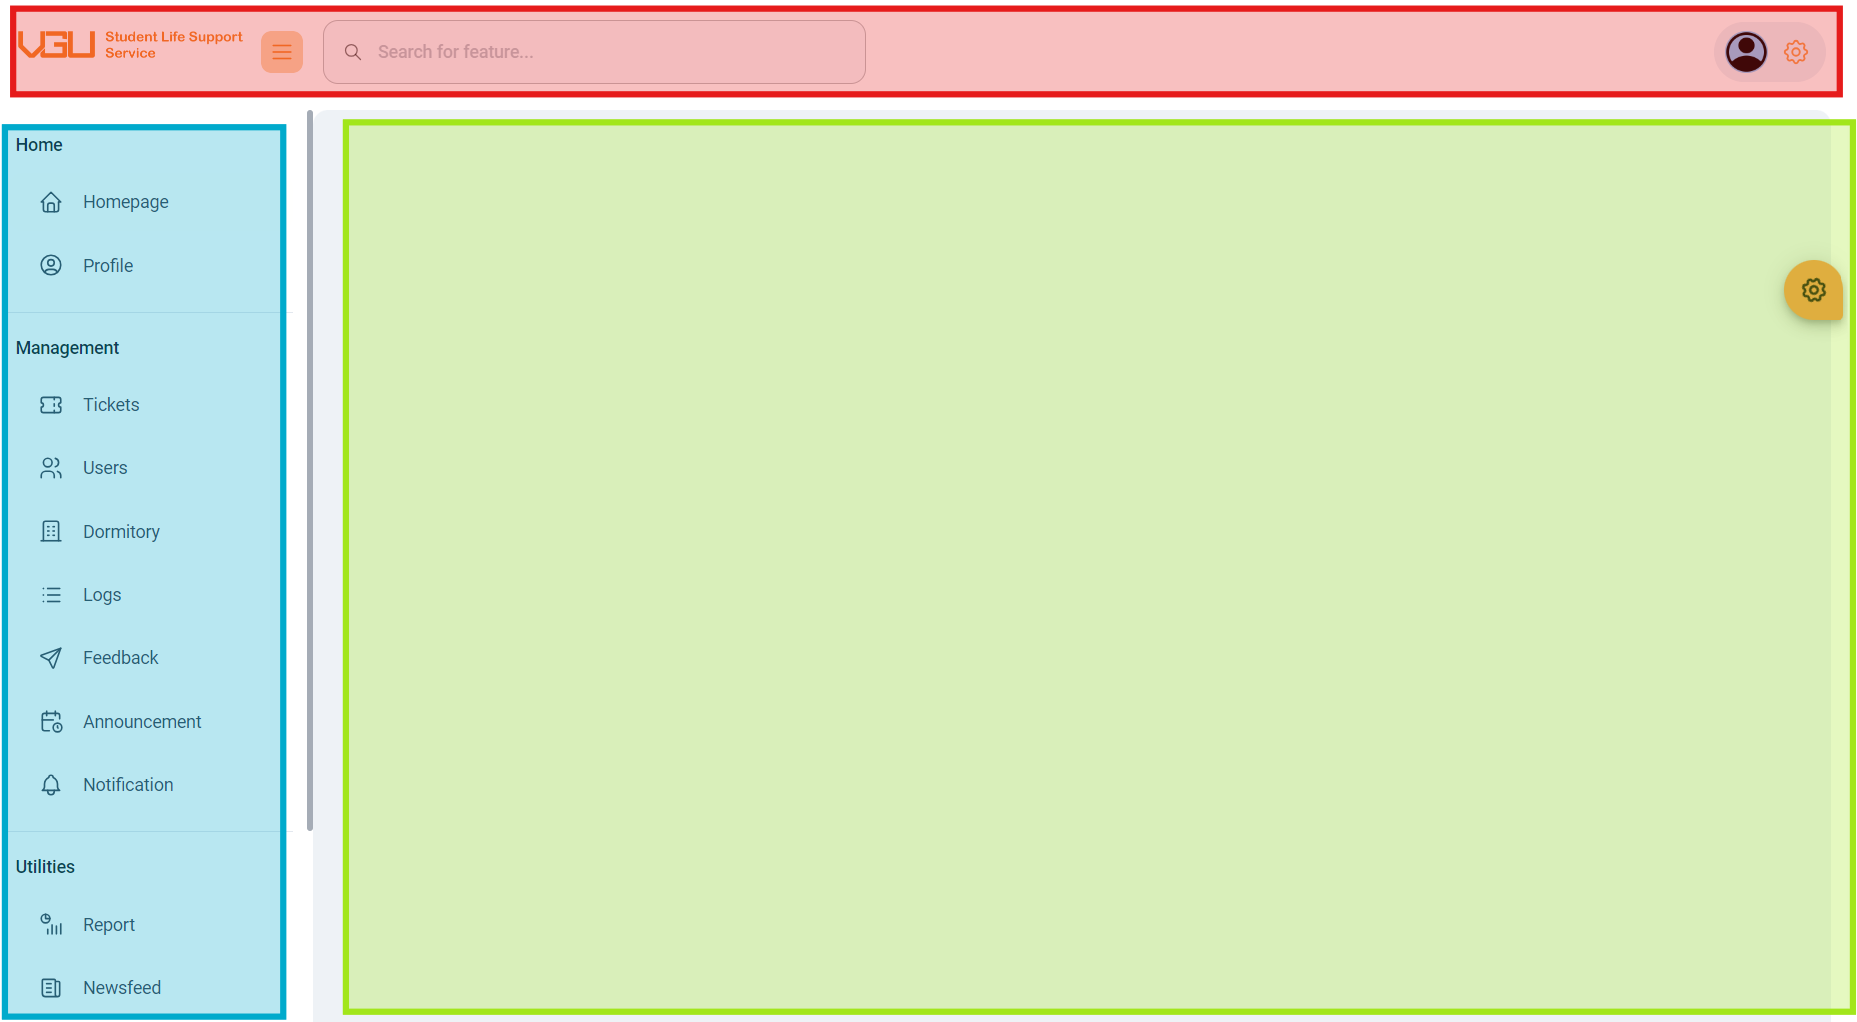
\includegraphics[width=1\linewidth]{graphics/fe/fe-main-comp}
		\caption{Web UI Main Components}
		\label{fig:fe-main-comp}
	\end{figure}
	There are 3 main components in the Web UI (from Figure \ref{fig:fe-main-comp}):
	
	\begin{enumerate}
		\item 	\colorbox{Salmon}{Header}: contains Logo image, Menu toggle button, Search bar, and Profile section  across all pages
		
\begin{lstlisting}[language=Javascript, breaklines=true, caption=Frontend Header Component]
const Header = ({ handleLeftDrawerToggle }) => {
	const theme = useTheme();
	
	return (
	<>
	{/* logo & toggler button */}
	<Box
	sx={{
			width: 228,
			display: 'flex',
			[theme.breakpoints.down('md')]: {
				width: 'auto'
			}
	}}
	>
	<Box component="span" sx={{ display: { xs: 'none', md: 'block' }, flexGrow: 1 }}>
	<LogoSection />
	</Box>
	<ButtonBase sx={{ borderRadius: '8px', overflow: 'hidden' }}>
	<Avatar
	variant="rounded"
	sx={{
			...theme.typography.commonAvatar,
			...theme.typography.mediumAvatar,
			transition: 'all .2s ease-in-out',
			background: theme.palette.secondary.light,
			color: theme.palette.secondary.dark,
			'&:hover': {
				background: theme.palette.secondary.dark,
				color: theme.palette.secondary.light
			}
	}}
	onClick={handleLeftDrawerToggle}
	color="inherit"
	>
	<IconMenu2 stroke={1.5} size="1.3rem" />
	</Avatar>
	</ButtonBase>
	</Box>
	
	{/* header search */}
	<SearchSection />
	<Box sx={{ flexGrow: 1 }} />
	<Box sx={{ flexGrow: 1 }} />
	

	{/* <ProfileSection /> */}
	<ProfileSection />
	</>
	);
};

Header.propTypes = {
	handleLeftDrawerToggle: PropTypes.func
};

export default Header;
\end{lstlisting}
		
		\item 	\colorbox{Aquamarine}{Sidebar}: A dynamic navigation panel which renders all menu items of a specific roles.
		
\begin{lstlisting}[language=Javascript, breaklines=true, caption=Frontend Sidebar Component]
const Sidebar = ({ drawerOpen, drawerToggle, window }) => {
	const theme = useTheme();
	const matchUpMd = useMediaQuery(theme.breakpoints.up('md'));
	
	const drawer = (
	<>
	<Box sx={{ display: { xs: 'block', md: 'none' } }}>
	<Box sx={{ display: 'flex', p: 2, mx: 'auto' }}>
	<LogoSection />
	</Box>
	</Box>
	
	<BrowserView>
	<PerfectScrollbar
	component="div"
	style={{
			// height: !matchUpMd ? 'calc(100vh - 56px)' : 'calc(100vh - 88px)',
			height: !matchUpMd ? 'calc(100vh - 56px)' : 'calc(100vh - 88px)',
			paddingLeft: '16px',
			paddingRight: '16px'
	}}
	>
	<MenuList />
	{/* <MenuCard /> */}
	<Stack direction="row" justifyContent="center" sx={{ mb: 2 }}>
	<Chip label="v1.0.0" disabled chipcolor="secondary" size="small" sx={{ cursor: 'pointer' }} />
	</Stack>
	</PerfectScrollbar>
	</BrowserView>
	
	<MobileView>
	<Box sx={{ px: 2 }}>
	<MenuList />
	{/* <MenuCard /> */}
	<Stack direction="row" justifyContent="center" sx={{ mb: 2 }}>
	<Chip label="v1.0.0" disabled chipcolor="secondary" size="small" sx={{ cursor: 'pointer' }} />
	</Stack>
	</Box>
	</MobileView>
	
	</>
	);
\end{lstlisting}		
		
		
		
		
		
		\item  \colorbox{YellowGreen}{Content Components}: The content component will be displayed based on the matched predefined route. Once the route is determined, the content component is then lazy-loaded into the page. This means that the component will only be fetched and rendered when it is needed, which optimizes performance and improves loading times by minimizing the amount of initial content loaded.
		
		
\begin{lstlisting}[language=Javascript, breaklines=true, caption=Example of Lazy Load Frontend Components]
const DashboardDefault = Loadable(lazy(() => import('views/homepage')));
const EditProfile = Loadable(lazy(() => import('views/EditProfile')));
const MyTickets = Loadable(lazy(() => import('views/MyTickets')));
\end{lstlisting}	
		
	\end{enumerate}
	
	
	\subsubsection{Responsive Design Implementation}
	Using Material-UI's grid system, responsive components, and utility features enables us to create a flexible and adaptive user interface in React applications. This ensures that the Web UI looks good and functions well on devices of all sizes, enhancing the overall user experience.
	
	\begin{enumerate}
		\item Grid System:
		
		MUI provides a powerful Grid component that allows us to create responsive layouts easily. It uses a 12-column layout, and we can specify how many columns a component should span at different screen sizes.


\begin{lstlisting}[language=Javascript, breaklines=true, caption=MUI Grid System]
import { Grid } from '@mui/material';

	<Grid container spacing={2}>
		<Grid item xs={12} sm={6} md={4}>
			<Card>Content 1</Card>
		</Grid>
		
		<Grid item xs={12} sm={6} md={4}>
			<Card>Content 2</Card>
		</Grid>
	
		<Grid item xs={12} md={4}>
			<Card>Content 3</Card>
		</Grid>
	</Grid>
\end{lstlisting}		

	\item Media Queries:
	
	MUI allows us to utilize CSS media queries through the sx prop or styles to create responsive designs that adapt to different screen sizes without much hassle.

\begin{lstlisting}[language=Javascript, breaklines=true, caption=MUI Media Queries]
<Box sx={{ 
		display: { xs: 'block', sm: 'flex' }, 
		flexDirection: { xs: 'column', sm: 'row' } 
}}>
{/* Our content */}
</Box>

\end{lstlisting}	


		
	\end{enumerate}

\subsection{Backend Implementation}
	\subsubsection{Source code structure}
	
	\begin{longtable}{{|m{4.8cm}|m{9.6cm}|}} 
		\hline
		\textbf{Module/component name} & \textbf{Description}\\ \hline
		
		config/ & contains server configurations, database connection class, constants.\\ \hline
		
		controllers/ & contains API controllers.\\ \hline
		
		middleware/ & contains server middleware (token authentication, logger, mailer). \\ \hline
		
		routes/ & defines explicit API routes  \\ \hline
		
		sql/ & contains all SQL queries. \\ \hline
		
		uploads/ & saves the user's uploaded attachments\\ \hline
		
		utils/ & contains shared utilities across modules \\ \hline
		
		index.js & root (start module) module of the backend server \\ \hline
		
		package.json & contains custom scripts and backend packages information \\ \hline
		
		.env & contains sensitive backend configurations \\ \hline
		
		\caption{Backend source code structure} % needs to go inside longtable environment
		\label{tab:be-src-code}
	\end{longtable}
	
	
	\subsubsection{Setting up ExpressJs Server}
	The implementation below sets up a web server with essential middleware and route handling for a robust application. It initializes the app, enabling JSON parsing, cookie parsing, and Cross-Origin Resource Sharing (CORS) with restricted options. The server then defines various API endpoints for authentication and resource management, including user, dorm, ticket, attachment, rating, message, role, notification, announcement, feedback, logs, and reports. Each route corresponds to a specific functionality, organized under the /auth and /api/v1/ prefixes, ensuring a structured and scalable approach to managing the application’s various services.

\begin{lstlisting}[language=Javascript, breaklines=true, caption=ExpressJS Server Setup]
const app = express();
app.use(express.json());
app.use(cookieParser()); // Enable cookie parsing
app.use(cors(WebConfig.corsOptions));


// ==============================|| Routes ||============================== //
app.use("/auth", authRoutes);                     
app.use("/api/v1/users", userRoutes);                  
app.use("/api/v1/dorms", dormRoutes)
app.use("/api/v1/tickets", ticketRoutes);        
app.use("/api/v1/attachments", attachmentRoutes); 
app.use("/api/v1/rating", ratingRoutes);          
app.use("/api/v1/messages", messageRoutes);
app.use("/api/v1/roles", roleRoutes);       
app.use("/api/v1/notification", notificationRoutes); 
app.use("/api/v1/announcement", announcementRoutes);        
app.use("/api/v1/feedback", feedbackRoutes);       
app.use("/api/v1/logs", logsRoutes);     
app.use("/api/v1/reports", reportRoutes);
\end{lstlisting}	

	\subsubsection{Database Integration}
	
\begin{lstlisting}[language=Javascript, breaklines=true, caption=Server connects to PostgreSQL Database]
import pkg from 'pg';
import dotenv from 'dotenv';

dotenv.config();

const { Pool } = pkg;

const pool = new Pool({
	user: String(process.env.PG_DB_USER),
	host: String(process.env.PG_DB_HOST),
	password: String(process.env.PG_DB_PASSWORD),
	port: Number(process.env.PG_DB_PORT),
	database: String(process.env.PG_DB_DATABASE),
});

export default pool;  
\end{lstlisting}	


\begin{lstlisting}[language=Javascript, breaklines=true, caption=Server connects to Redis]
import redis from 'redis';

const redisClient = redis.createClient({
	socket: {
		host: process.env.REDIS_HOST,
		port: process.env.REDIS_PORT,
	},
});


const connectRedis = async () => {
	await redisClient.connect();
	redisClient.on('error', (err) => {
		console.error('Redis error:', err);
	});
	console.log('Redis connected successfully');
};
\end{lstlisting}	


\subsubsection{Security Measures}


	
	
	